\section{HPCG}
\subsection{One-node performance}
S'ha mesurat la performance del benchmark HPCG, el qual la reporta en GFlops, en un node. 

S'han obtingut dades executant en un node amb diferents combinacions de MPI ranks i threads. En el cas d'1 procés, s'ha afegit l'execució amb 16 threads. D'aquesta manera s'arriba a omplir el node, com en el cas de 2 processos i 8 threads.

% scalability 
\begin{table}[]
    \centering
\begin{tabular}{ccc}
    \hline
    Processes           & Threads                    & Avg GFlops                   \\ \hline \hline
                        & \cellcolor[HTML]{EFEFEF}1  & \cellcolor[HTML]{EFEFEF}1.13 \\
                        & 2                          & 1.21                         \\
                        & \cellcolor[HTML]{EFEFEF}4  & \cellcolor[HTML]{EFEFEF}1.30 \\
                        & 8                          & 1.32                         \\
    \multirow{-5}{*}{1} & \cellcolor[HTML]{EFEFEF}16 & \cellcolor[HTML]{EFEFEF}1.30 \\ \hline
                        & 1                          & 2.08                         \\
                        & \cellcolor[HTML]{EFEFEF}2  & \cellcolor[HTML]{EFEFEF}2.35 \\
                        & 4                          & 2.42                         \\
    \multirow{-4}{*}{2} & \cellcolor[HTML]{EFEFEF}8  & \cellcolor[HTML]{EFEFEF}2.49 \\ \hline
    \end{tabular}
    \caption{Performance amb diferents ranks i threads.}
    \label{tab:hpcg_global_perf}
\end{table}

\begin{figure}
    \centering
    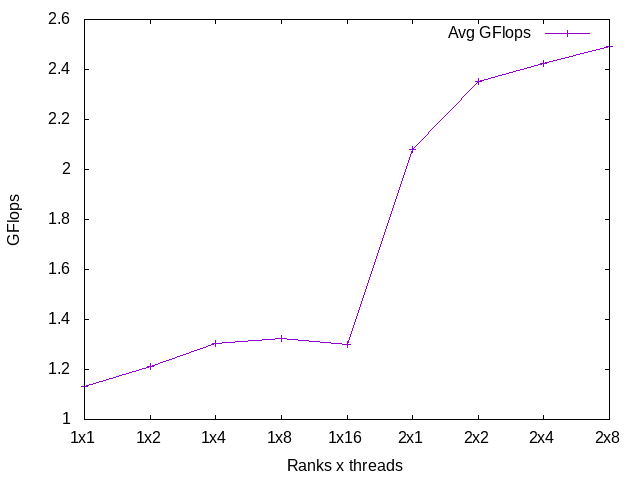
\includegraphics[width=0.5\textwidth]{img/hpcg_global_grafica.png}
    \caption{Gràfica de la performance global.}
    \label{fig:hpcg_global_perf}
\end{figure}

A la taula \ref{tab:hpcg_global_perf} es poden observar els resultats obtinguts, els quals estan representats en la gràfica \ref{tab:hpcg_global_perf}. Es pot observar que afegint threads HPCG no escala bé. En canvi, afegint processos escala millor, tal com es pot veure comparant els GFlops que s'obtenen executant el mateix nombre de CPUs, però amb diferent nombre de processos i threads. Per exemple, observant la performance amb 1 procés i 2 threads, i amb 2 ranks i 1 thread, es veu una diferencia d'aproximadament 1 GFlop.

Aquest benchmark no escala bé utilitzant threads perquè té molt poca regió de codi paral·lelitzada amb OpenMP. 
Es recomana la lectura de la publicació de D. Ruiz \textit{et al.} \cite{ruiz_hpcg_nodate}, sobre la millora de la performance d'aquest d'HPCG gràcies a la paral·lelització d'una de les funcions amb més pes a l'execució mitjançant OpenMP. 
El codi resultant, i posteriors optimitzacions, està disponible en un repositori d'ARM 
\footnote{Repositori de la versió d'ARM d'HPCG \url{https://gitlab.com/arm-hpc/benchmarks/hpcg}}.


% --------------------------------------------------------------------------------------------
\subsection{Kernels}
El benchmark està composat per diferents kernels: DDOT, WAXPBY, SpMV i MG. 

El que més pes té a l'execució és MG. Es pot observar a la taula \ref{tab:hpcg_kernel_perf} com els seus GFlops són molt propers als GFlops globals que reporta HPCG. 
Això ens indica que aquesta funció està paral·lelitzada amb MPI i no OpenMPI, o molt poc. Es pot veure a la gràfica \ref{fig:hpcg_kernels_grafica} que no escala. 
Els kernels DDOT i WAXPBY segueixen una tendencia semblant, és a dir, poca escalabilitat afegint threads.

També es pot observar, tant a la taula \ref{tab:hpcg_kernel_perf} com a la gràfica \ref{fig:hpcg_kernels_grafica}, que l'únic kernel que escala al afegir threads és SpMV. Això suggereix que aquest kernel sí que està paral·lelitzat amb OpenMP.

Com es pot trobar en el paper mencionat anteriorment \cite{ruiz_hpcg_nodate}, a la figura 2, cada kernel té un percentatge de temps d'execució de:
\begin{itemize}
    \item DDOT:         1.05\%
    \item WAXPBY:       1.37\%
    \item SpMV:         12.61\%
    \item MG:           84.97\%
\end{itemize}
% scalability

\begin{table}[]
    \centering
    \begin{tabular}{cccc}
    \hline
Kernels                  & Processes                                   & Threads                    & Avg GFlops                        \\ \hline \hline
                         & \cellcolor[HTML]{EFEFEF}                    & \cellcolor[HTML]{EFEFEF}1  & \cellcolor[HTML]{EFEFEF}1.42702   \\
                         & \cellcolor[HTML]{EFEFEF}                    & 2                          & 1.193376                          \\
                         & \cellcolor[HTML]{EFEFEF}                    & \cellcolor[HTML]{EFEFEF}4  & \cellcolor[HTML]{EFEFEF}1.233166  \\
                         & \cellcolor[HTML]{EFEFEF}                    & 8                          & 1.041158                          \\
                         & \multirow{-5}{*}{\cellcolor[HTML]{EFEFEF}1} & \cellcolor[HTML]{EFEFEF}16 & \cellcolor[HTML]{EFEFEF}0.6321778 \\ \cline{3-4} 
                         &                                             & 1                          & 1.713664                          \\
                         &                                             & \cellcolor[HTML]{EFEFEF}2  & \cellcolor[HTML]{EFEFEF}1.888934  \\
                         &                                             & 4                          & 1.2960886                         \\
\multirow{-9}{*}{DDOT}   & \multirow{-4}{*}{2}                         & \cellcolor[HTML]{EFEFEF}8  & \cellcolor[HTML]{EFEFEF}1.2932232 \\ \hline
                         & \cellcolor[HTML]{EFEFEF}                    & 1                          & 1.299504                          \\
                         & \cellcolor[HTML]{EFEFEF}                    & \cellcolor[HTML]{EFEFEF}2  & \cellcolor[HTML]{EFEFEF}1.087426  \\
                         & \cellcolor[HTML]{EFEFEF}                    & 4                          & 1.337632                          \\
                         & \cellcolor[HTML]{EFEFEF}                    & \cellcolor[HTML]{EFEFEF}8  & \cellcolor[HTML]{EFEFEF}1.224306  \\
                         & \multirow{-5}{*}{\cellcolor[HTML]{EFEFEF}1} & 16                         & 0.88919                           \\ \cline{3-4} 
                         &                                             & \cellcolor[HTML]{EFEFEF}1  & \cellcolor[HTML]{EFEFEF}2.63542   \\
                         &                                             & 2                          & 2.299548                          \\
                         &                                             & \cellcolor[HTML]{EFEFEF}4  & \cellcolor[HTML]{EFEFEF}2.54233   \\
\multirow{-9}{*}{WAXPBY} & \multirow{-4}{*}{2}                         & 8                          & 2.185762                          \\ \hline
                         & \cellcolor[HTML]{EFEFEF}                    & \cellcolor[HTML]{EFEFEF}1  & \cellcolor[HTML]{EFEFEF}1.357868  \\
                         & \cellcolor[HTML]{EFEFEF}                    & 2                          & 2.433688                          \\
                         & \cellcolor[HTML]{EFEFEF}                    & \cellcolor[HTML]{EFEFEF}4  & \cellcolor[HTML]{EFEFEF}4.477724  \\
                         & \cellcolor[HTML]{EFEFEF}                    & 8                          & 7.158042                          \\
                         & \multirow{-5}{*}{\cellcolor[HTML]{EFEFEF}1} & \cellcolor[HTML]{EFEFEF}16 & \cellcolor[HTML]{EFEFEF}8.492038  \\ \cline{3-4} 
                         &                                             & 1                          & 2.084098                          \\
                         &                                             & \cellcolor[HTML]{EFEFEF}2  & \cellcolor[HTML]{EFEFEF}3.961412  \\
                         &                                             & 4                          & 6.670772                          \\
\multirow{-9}{*}{SpMV}   & \multirow{-4}{*}{2}                         & \cellcolor[HTML]{EFEFEF}8  & \cellcolor[HTML]{EFEFEF}10.89098  \\ \hline
                         & \cellcolor[HTML]{EFEFEF}                    & 1                          & 1.168888                          \\
                         & \cellcolor[HTML]{EFEFEF}                    & \cellcolor[HTML]{EFEFEF}2  & \cellcolor[HTML]{EFEFEF}1.19261   \\
                         & \cellcolor[HTML]{EFEFEF}                    & 4                          & 1.250284                          \\
                         & \cellcolor[HTML]{EFEFEF}                    & \cellcolor[HTML]{EFEFEF}8  & \cellcolor[HTML]{EFEFEF}1.260128  \\
                         & \multirow{-5}{*}{\cellcolor[HTML]{EFEFEF}1} & 16                         & 1.251848                          \\ \cline{3-4} 
                         &                                             & 1                          & 2.228456                          \\
                         &                                             & \cellcolor[HTML]{EFEFEF}2  & \cellcolor[HTML]{EFEFEF}2.360568  \\
                         &                                             & 4                          & 2.400454                          \\
\multirow{-9}{*}{MG}     & \multirow{-4}{*}{2}                         & \cellcolor[HTML]{EFEFEF}8  & \cellcolor[HTML]{EFEFEF}2.420986  \\ \hline
    \end{tabular}
    \caption{Performance dels kernels.}
    \label{tab:hpcg_kernel_perf}
\end{table}


\begin{figure}
    \centering
    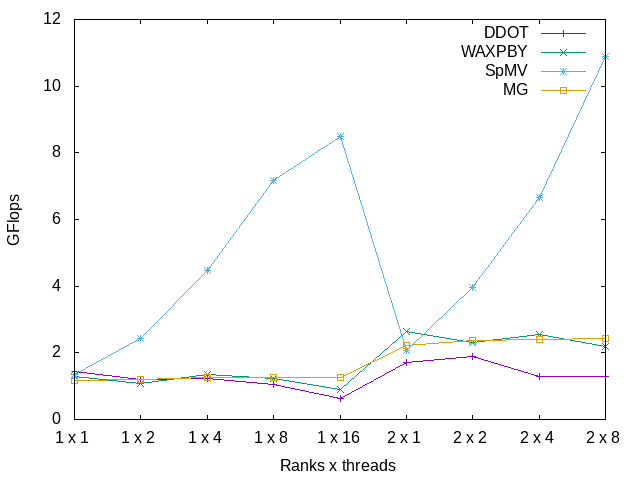
\includegraphics[width=0.5\textwidth]{img/hpcg_kernels_grafica.png}
    \caption{Gràfica de la performance de cada kernel.}
    \label{fig:hpcg_kernel_perf}
\end{figure}

\subsection{Comparativa amb Linpack}
